% Document Class is specified here. We're using the Homework Template
\documentclass[12pt, a4paper]{article}

\usepackage{graphicx}
\usepackage{float}
\usepackage{geometry}
\usepackage{verbatim}

\geometry{a4paper, margin=1in}

\title{Week 3 CS-312 Homework}
\author{
	Cory Ness
	\and
	Jack Engledow
	\and
	James Sgrazzutti
}

\begin{document}

\maketitle

\section{Problem 3.1}
\subsection{Question}
Give an NFA for the language of RE $a^{*}b+b^{*}a$
\subsection{Answer}
\begin{center}
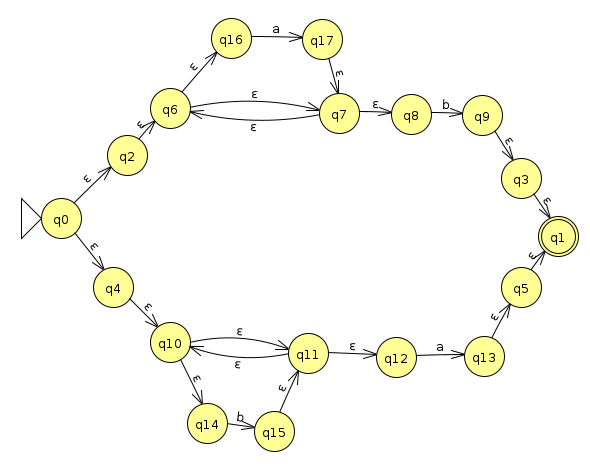
\includegraphics[scale=0.7]{3.1}
\end{center}

\section{Problem 3.6}
\subsection{Question}
Show how to modify an NFA to have a unique accept state with no transition ending at the start state and no transition starting at the accept state.
\subsection{Answer}
We'll begin with an NFA that fails both of these conditions, where there is a transition ending at the start state and a transition starting at multiple accept states.
\begin{center}
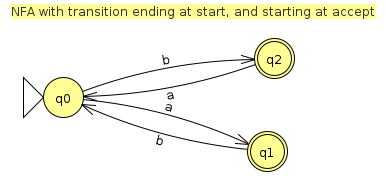
\includegraphics[scale=0.7]{3.6a}
\end{center}
To remove transitions that end at the start state, add another state that becomes the start state and transition to the old start state using $\epsilon$.
\begin{center}
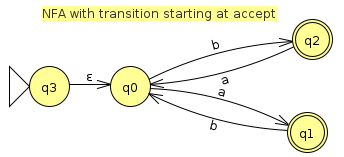
\includegraphics[scale=0.7]{3.6b}
\end{center}
To remove transitions that start at the end state, add another state the becomes a accept state, make all the old accept states non-accept states, and transition all the old accept states to the new accept state using $\epsilon$.
\begin{center}
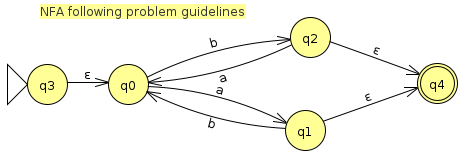
\includegraphics[scale=0.7]{3.6c}
\end{center}

\section{Problem 3.7}
\subsection{Question}
If $M$ is a DFA accepting language $B$, then exchanging the accept and reject states gives a new DFA accepting the complement of $B$. Does this work for an NFA? Discuss.
\subsection{Answer}
No, below is an NFA that accepts the string "1".
\begin{center}
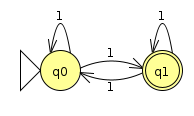
\includegraphics[scale=0.7]{3.7a}
\end{center}
And below is an NFA that also accepts the string "1", even though the accept and reject states were swapped.
\begin{center}
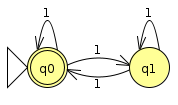
\includegraphics[scale=0.7]{3.7b}
\end{center}
This is because an NFA has the ability to transition through multiple possible states at the same time, so merely swapping the accept and reject states isn't sufficient, as an NFA may be in both an accept and reject state under normal circumstances.

\section{Problem 3.9}
\subsection{Question}
For the following NFA, use the subset construction to produce an equivalent DFA.
\begin{center}
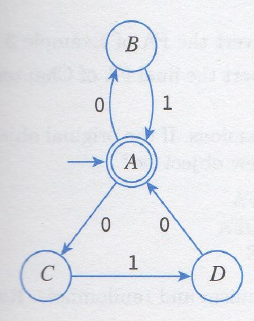
\includegraphics[scale=0.7]{3.9problem}
\end{center}
\subsection{Answer}
\begin{center}
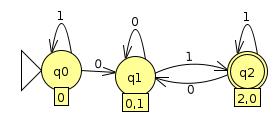
\includegraphics[scale=0.7]{3.9}
\end{center}

\section{Problem 3.11}
\subsection{Question}
Provide an algorithm to tell if the language is infinite if the input is
\subsubsection{An RE}
Find a Kleen Star (*) that proceeds a non-empty string. If one exists, the language is infinite since there can be any number of repetition of the preceding string.
\subsubsection{An NFA}
Find a loop through the NFA using Depth-First search. If in the process of searching, one of the ancestors in the tree was reached, there is a loop in the graph and the NFA is infinite because that loop can be repeated.

\section{Problem 4.1}
\subsection{Question}
Show that the set of regular languages is closed under reversal. That is, if $L$ is regular, then so is $\{x^{R} : x \in L\}$ where $x^{R}$ denotes the reversal of string $x$.
\subsection{Answer}
To prove that the set of regular languages is closed under reversal, we can look at a Finite Automata equivalent of each language where there is a single start state and a single end state, which was proven to always be able to be constructed in problem 3.6. From here, we can perform our reversal operation, which includes swapping the start state and end state, and swapping the direction of every transition between states. This produces another Finite Automata that has undergone the reversal operation, hence a regular language. This means that the set of regular languages is closed under reversal.

\section{Problem 4.11}
\subsection{Question}
Show that $\{x\#x : x \in \{0,1\}^{*}\}$ is non regular. (The hash mark/pound sign is a special symbol that should only occur in the middle of the input string.)
\subsection{Answer}
This expression is non regular for much the same reason that $0^{n}1^{n}$ in non regular. Since the Hash symbol must be in the exact middle of the expression, the Finite Automaton must count the number of symbols preceding the symbol and compare it to the number of symbols succeeding it. Since an acceptable string can be arbitrarily long, there must be an infinite number of states for the Finite Automaton. Since this is impossible, it must be concluded that the expression $\{x\#x : x \in \{0,1\}^{*}\}$ is non regular.

\section{Problem 4.13b}
\subsection{Question}
State whether the set of binary non palindromes is regular or not. If not, give a proof that it is non regular.
\subsection{Answer}
The set of binary non palindromes is the complement of the set of palindromes. Since the set of regular languages is closed under the complement, if we can prove that palindromes are regular, we can prove that non palindromes are also regular.

The set of palindromes is not regular due to the Pumping Lemma theorem. Take the expression $\{a^{n}bba^{n} : a \in \{0,1\}^{*}, b \in \{0,1\}^{*}\}$. Where $w=uvx$, and $uv \leq n$. Since $v \geq 1$, we can conclude that v is composed entirely of some subset of the first a. By the Pumping Lemma, we must conclude that $ux$ is also a part of the expression, but it cannot be so because some part of $a$ is missing in the first half, so palindromes are not regular.

\section{Problem 4.14}
\subsection{Question}
Explain what is wrong with the following "proof" that the language $L$ of an RE $a^{*}b^{*}$ is non regular.

\begin{quotation}
Suppose $L$ were regular. Then it would be accepted by a DFA with, say, $k$ states. Consider the string $z=0^{k}1^{k}$. Split $z=uvw$ with $v=01$. Then $uv^{2}w$ is not in $L$. This is a contradiction of the Pumping Lemma, and so our supposition is false.
\end{quotation}
\subsection{Answer}
This proof is wrong because it proved that a subset of expressions define by $a^{*}b^{*}$ is non regular, thinking it would prove the general case. A regular language can contain non regular expressions, which the proof showed, but it did not show that the language itself is non regular.

\section{Problem 4.20}
\subsection{Question}
Convince your grandmother that there is no FA that accepts the language of binary strings with an equal number of $0$'s and $1$'s.
\subsection{Answer}
The definition of a Finite Automata is that it contains a fixed number of states.
In order to keep track of count in a Finite Automata, there must be a unique state for each count of some thing, as in a state for 1 item, a state for 2 items, a state for 3 items, etc.
The string passed into a Finite Automata can be arbitrarily large, even infinite.
In order to accept a language that has the same number of $0$'s and $1$'s, the Finite Automata must count the number of $0$'s and compare it to the number of $1$'s.
Since the string can be arbitrarily large, and an arbitrarily large string can be accepted by this expression, the Finite Automata must count an arbitrarily large number of $0$'s and $1$'s.
Because of this, the Finite Automata must have an arbitrarily large, even infinite, number of states.
A Finite Automata cannot have an infinite number of states, so it cannot accept the language of binary strings with an equal number of $0$'s and $1$'s.


\end{document}